\documentclass[11pt,epsf,times,letterpaper]{article}
\usepackage[spanish]{babel}
\usepackage[latin1]{inputenc}
\usepackage{amsmath}
\usepackage{graphicx}
\usepackage{array}
\usepackage{enumerate}
\usepackage{fullpage}

\begin{document}
	
	\begin{figure}
		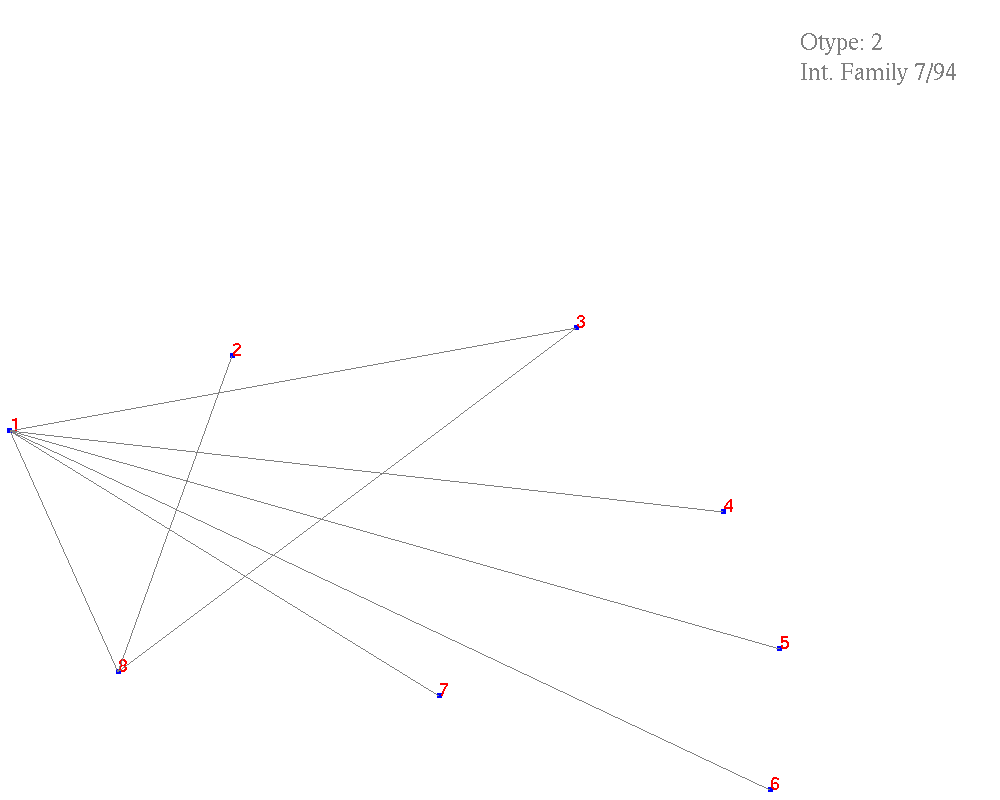
\includegraphics[scale=.4]{if_tam0_tam1/1.png}
		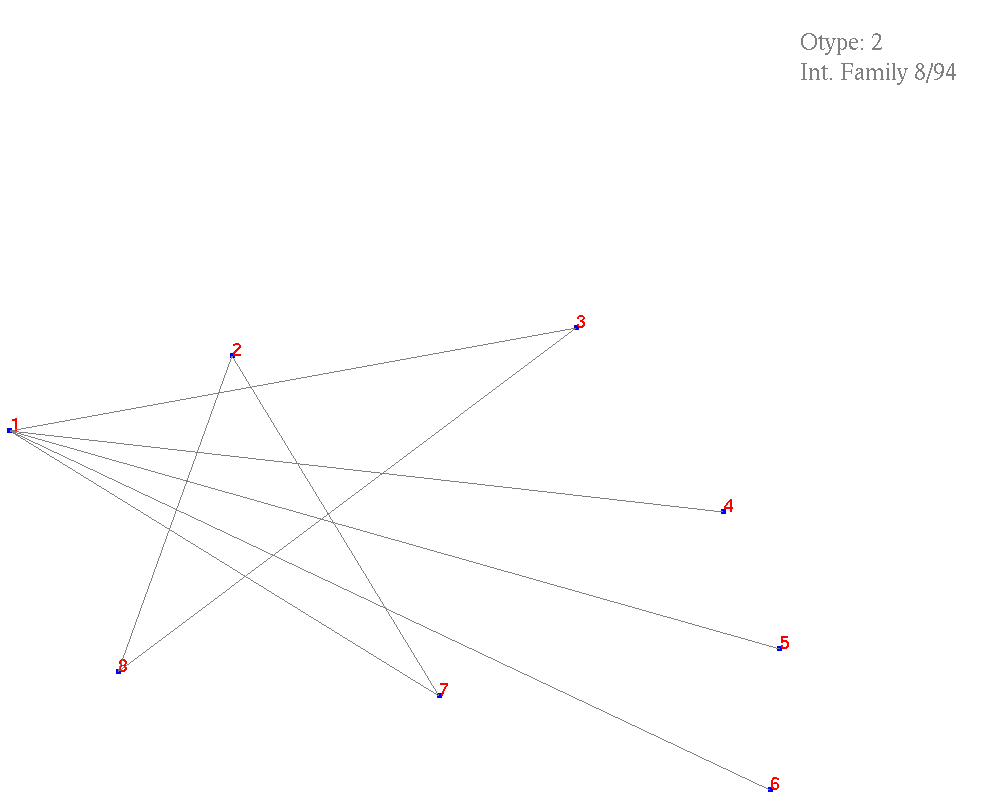
\includegraphics[scale=.4]{if_tam0_tam1/2.png}
	\end{figure}

	\begin{figure}
		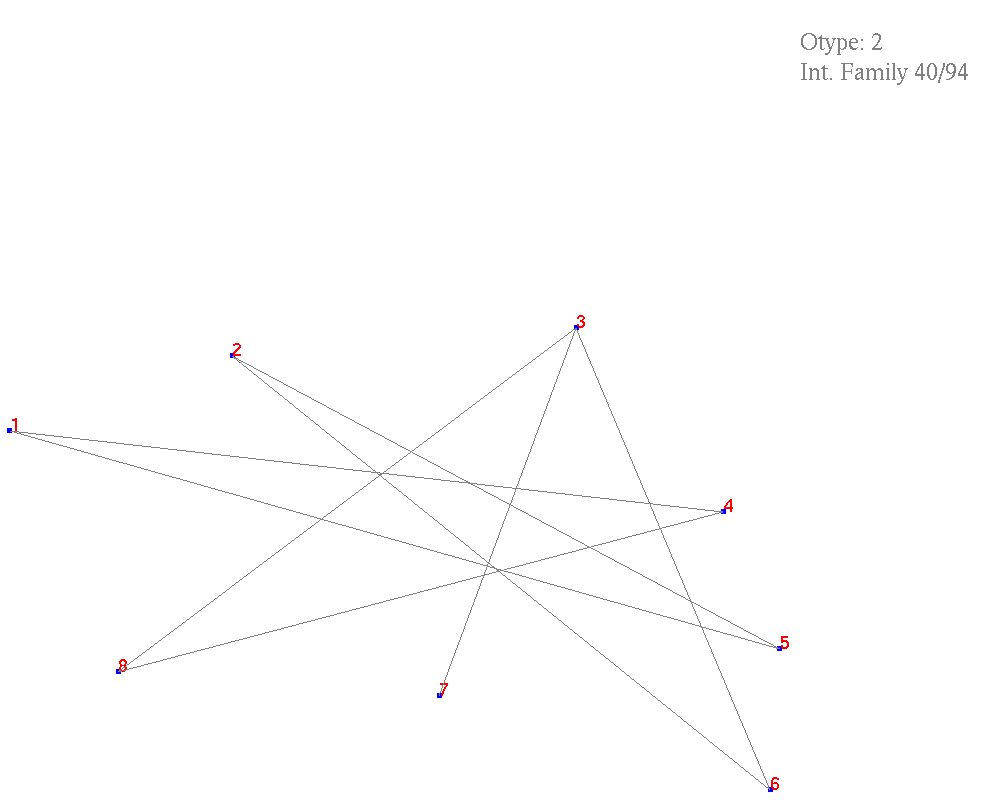
\includegraphics[scale=.4]{if_tam0_tam1/3.png}
		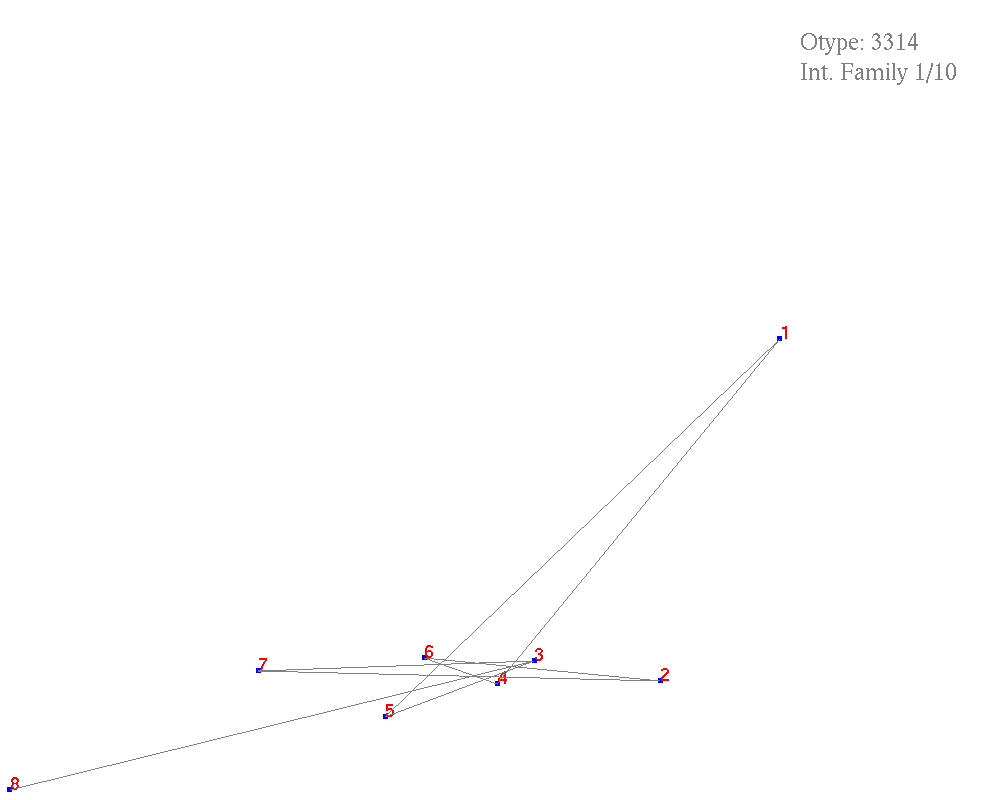
\includegraphics[scale=.4]{if_tam0_tam1/4.png}
	\end{figure}
	
	\begin{figure}
		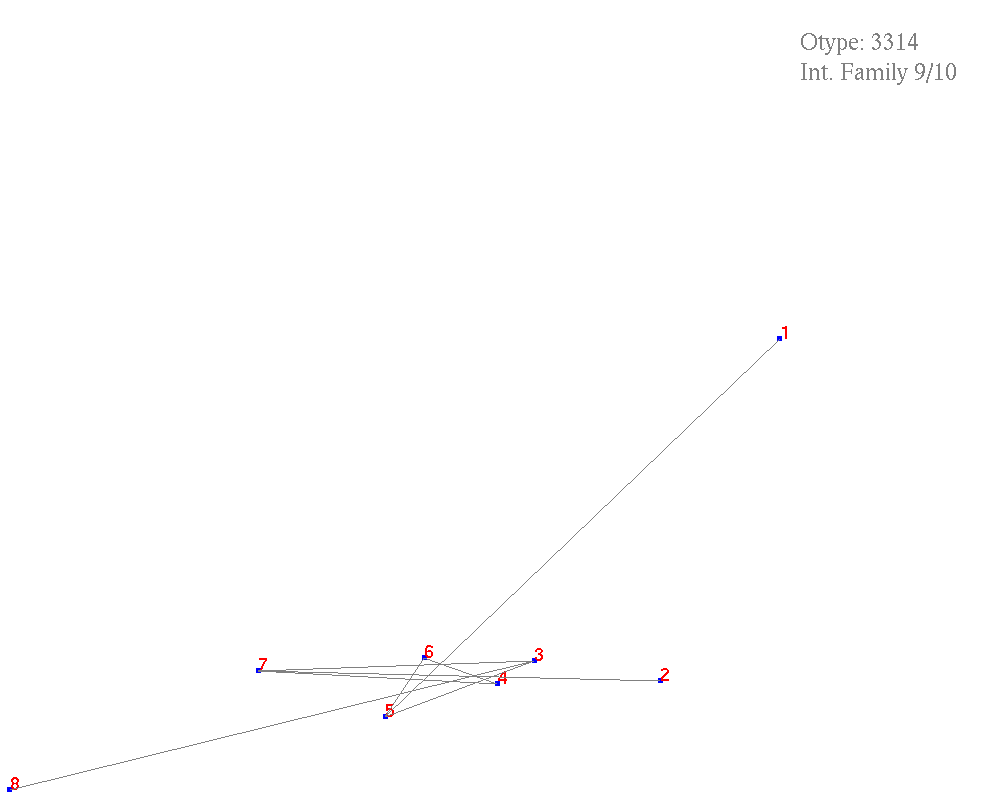
\includegraphics[scale=.4]{if_tam0_tam1/5.png}
		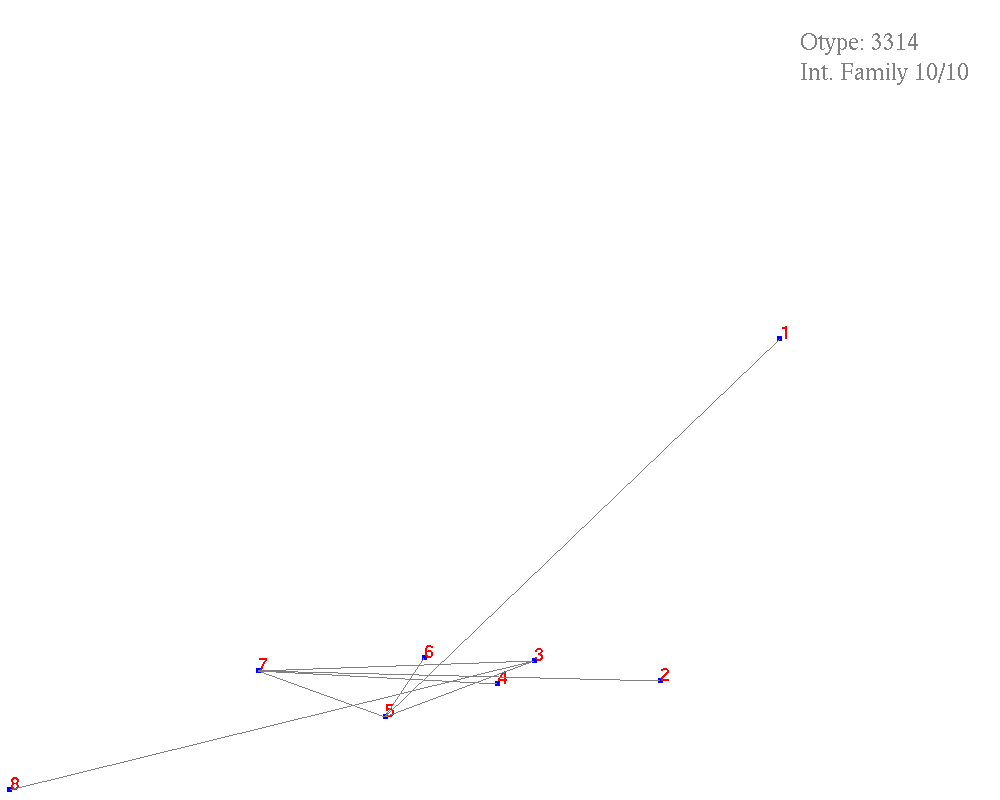
\includegraphics[scale=.4]{if_tam0_tam1/6.png}
	\end{figure}
	
	\begin{figure}
		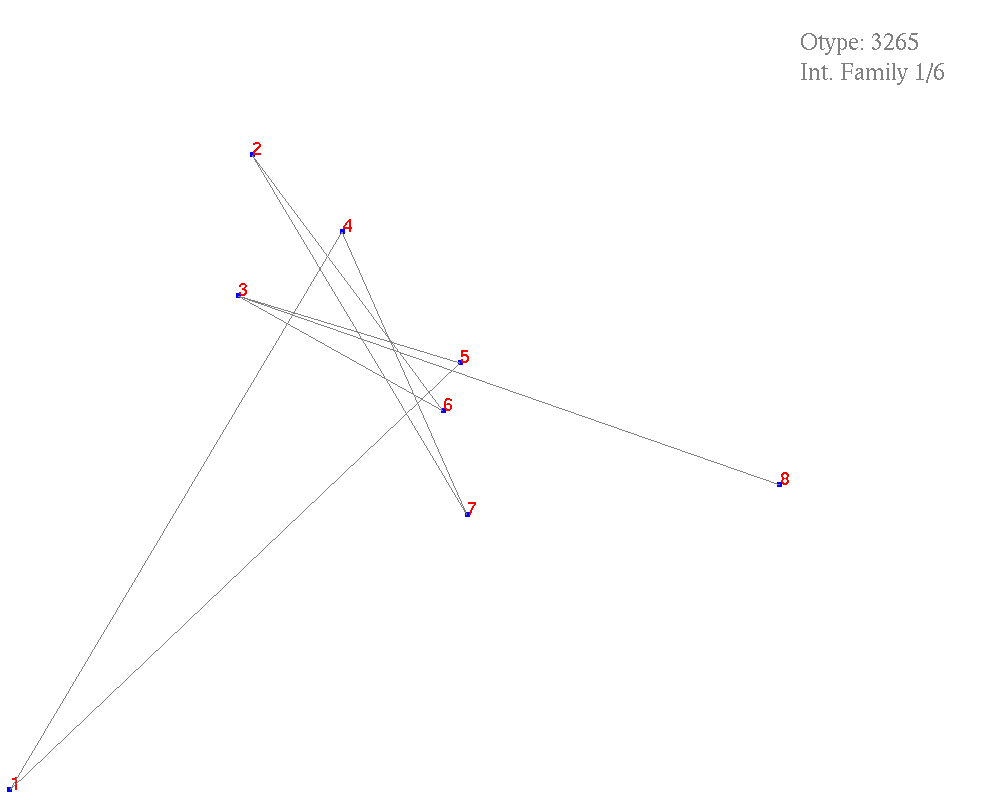
\includegraphics[scale=.4]{if_tam0_tam1/7.png}
		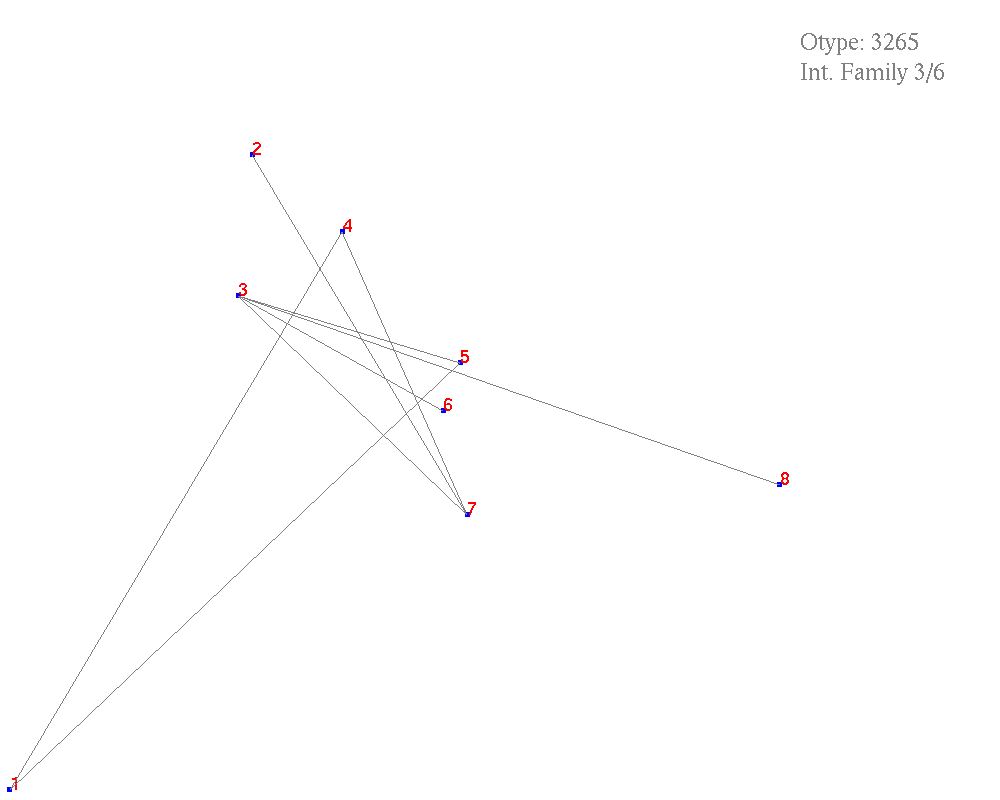
\includegraphics[scale=.4]{if_tam0_tam1/8.png}
	\end{figure}
	
	\begin{figure}
		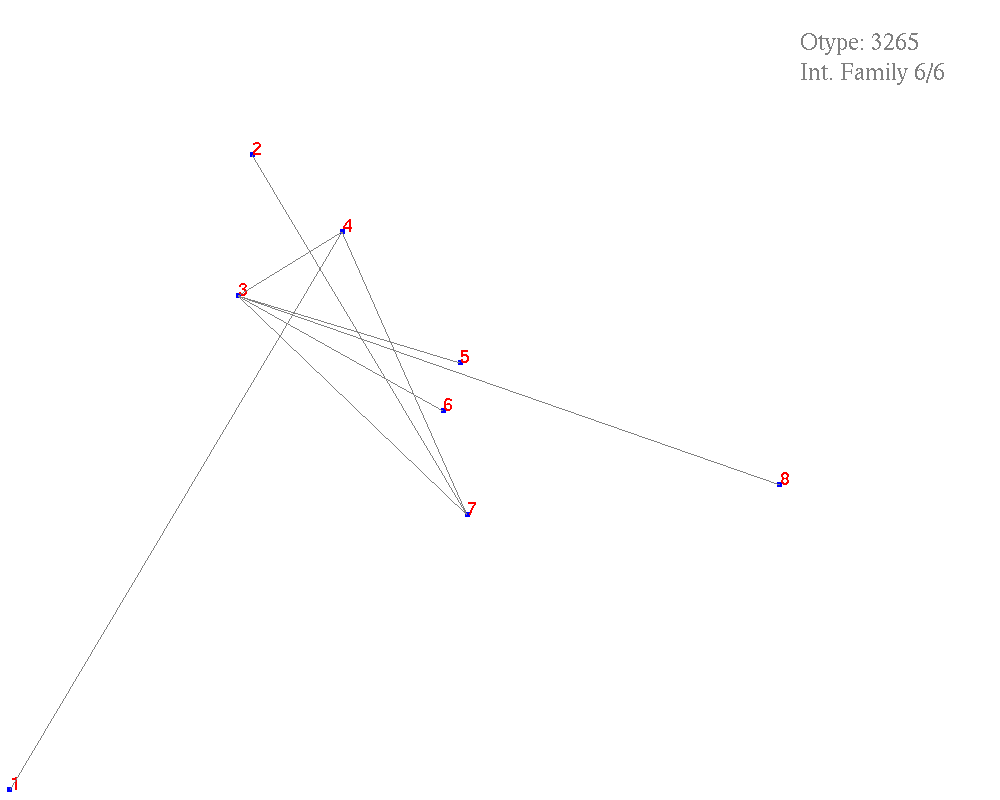
\includegraphics[scale=.4]{if_tam0_tam1/9.png}
		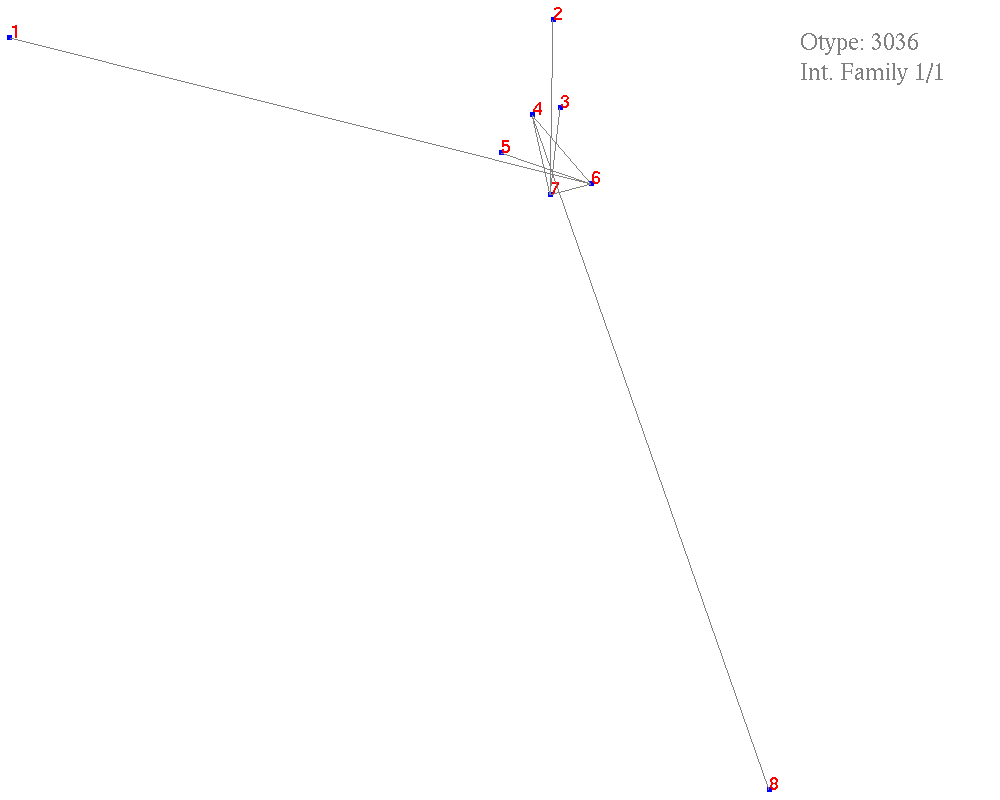
\includegraphics[scale=.4]{if_tam0_tam1/10.png}
	\end{figure}
	
	\begin{figure}
		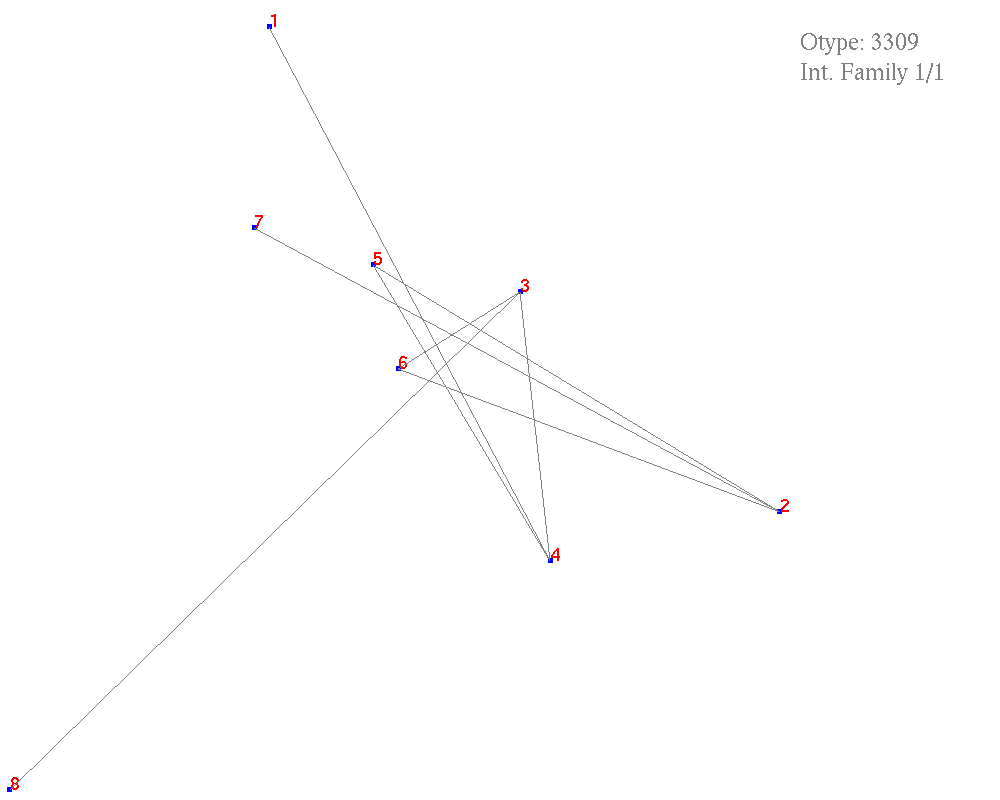
\includegraphics[scale=.4]{if_tam0_tam1/11.png}
		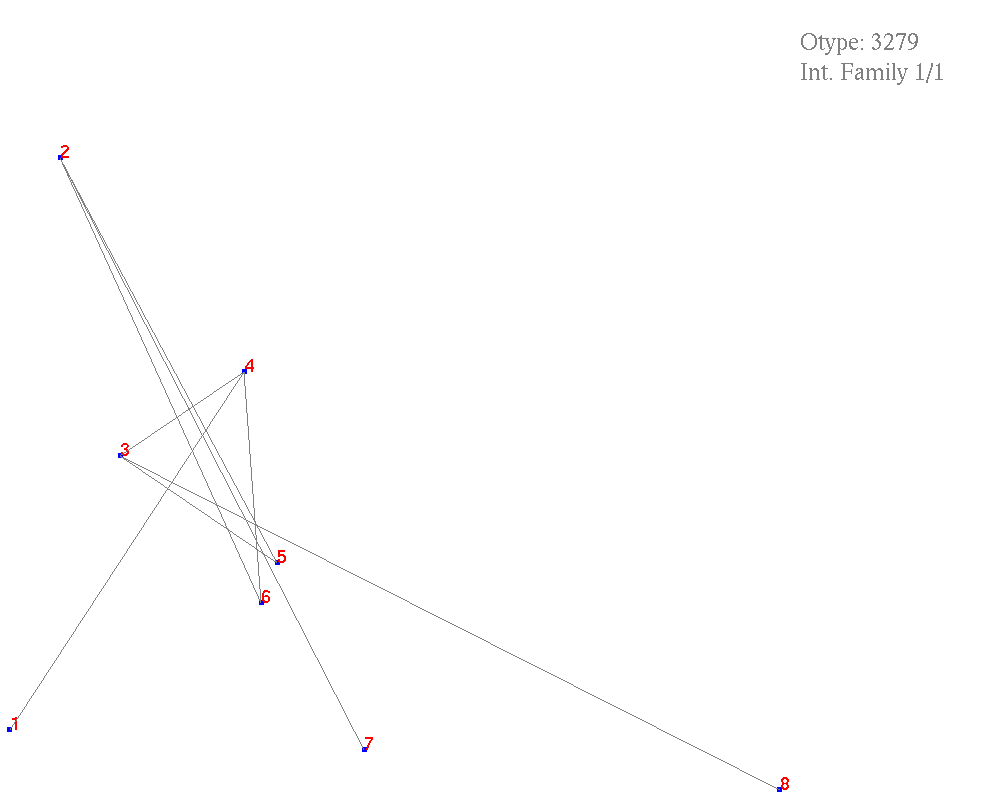
\includegraphics[scale=.4]{if_tam0_tam1/12.png}
	\end{figure}
	\begin{figure}
		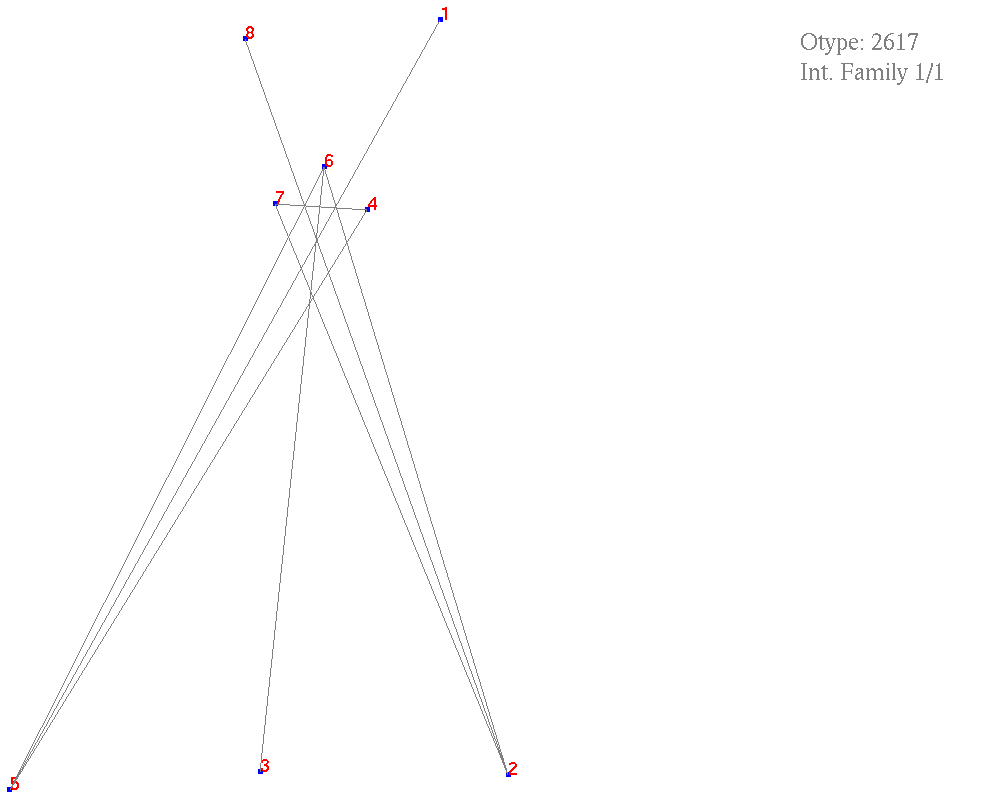
\includegraphics[scale=.4]{if_tam0_tam1/13.png}
		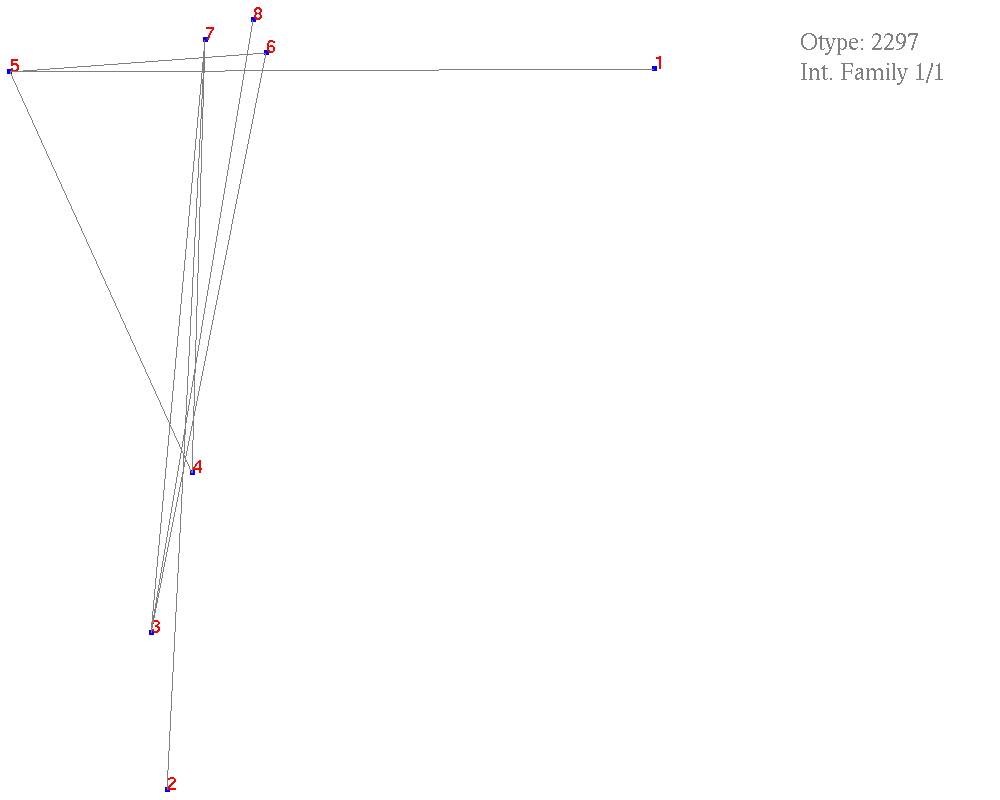
\includegraphics[scale=.4]{if_tam0_tam1/14.png}
	\end{figure}
		
	\begin{figure}
		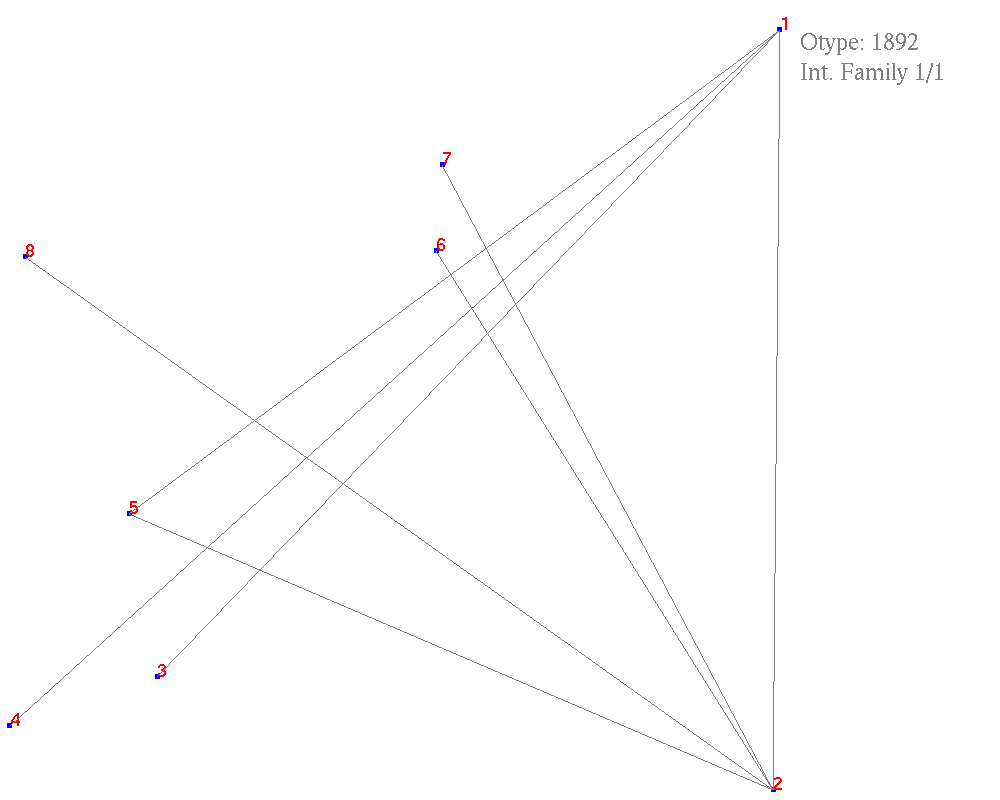
\includegraphics[scale=.4]{if_tam0_tam1/15.png}
		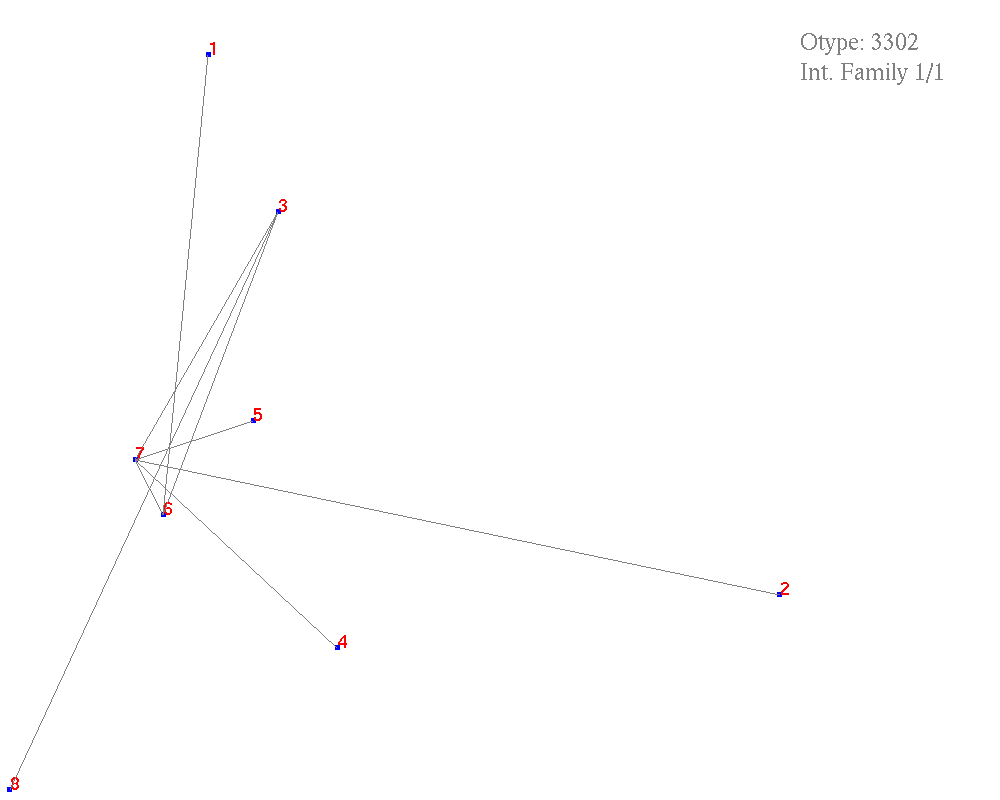
\includegraphics[scale=.4]{if_tam0_tam1/16.png}
	\end{figure}
	
	\begin{figure}
		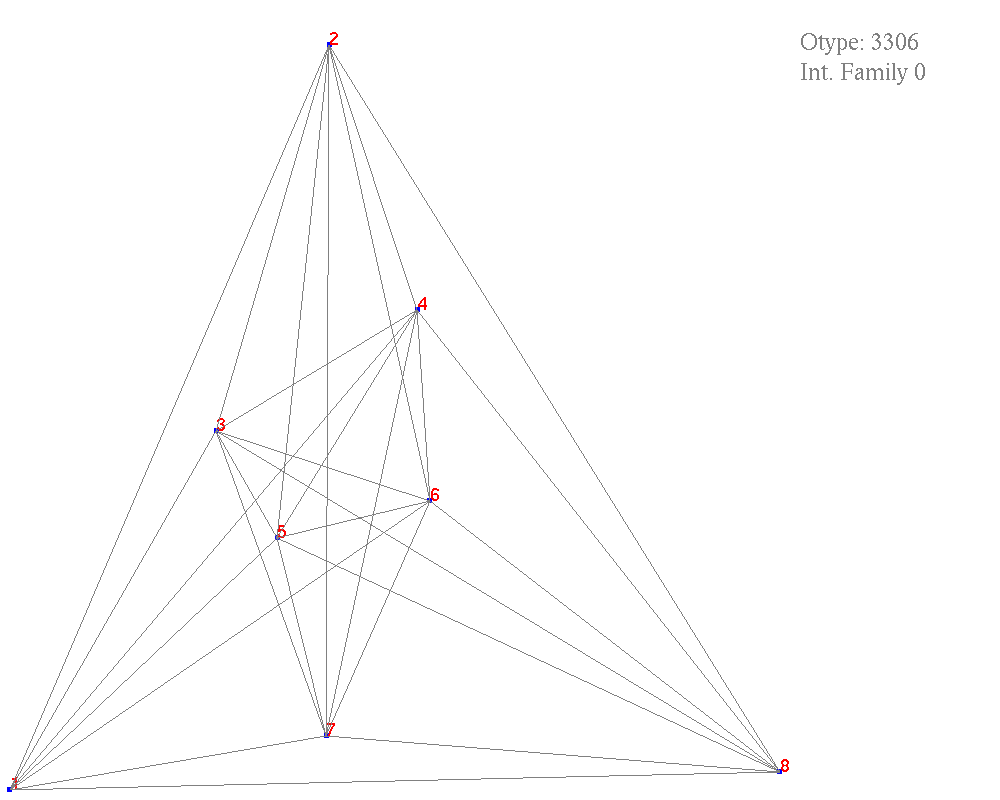
\includegraphics[scale=.4]{if_tam0_tam1/17.png}
		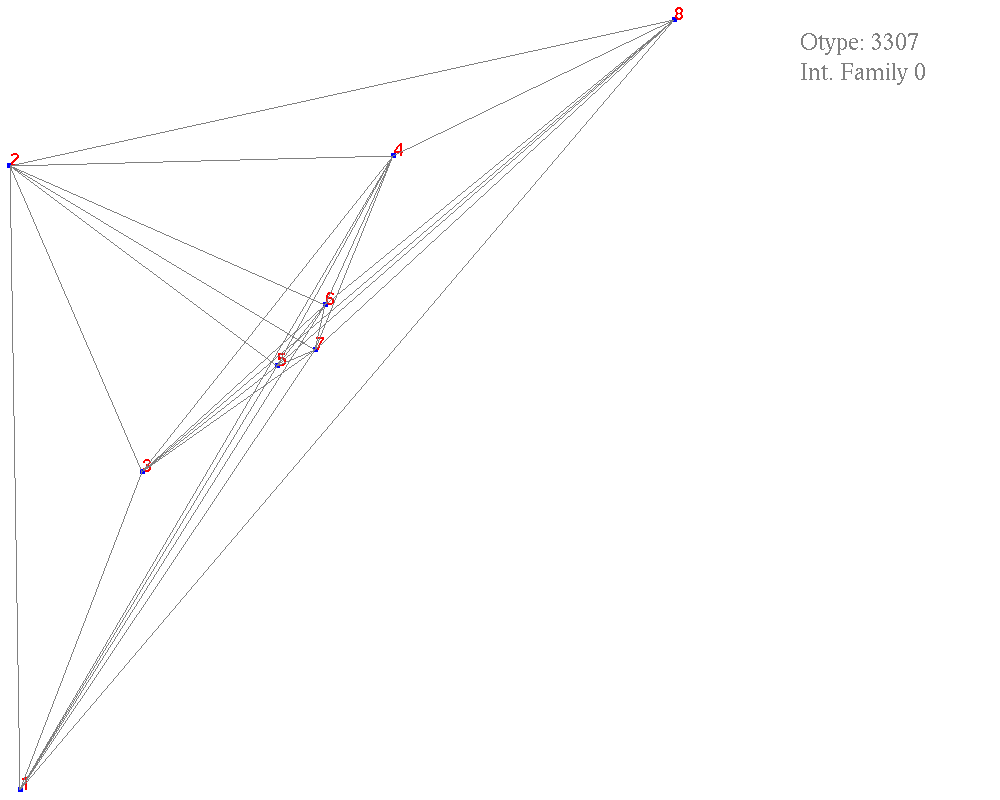
\includegraphics[scale=.4]{if_tam0_tam1/18.png}
	\end{figure}
	
	\begin{figure}
		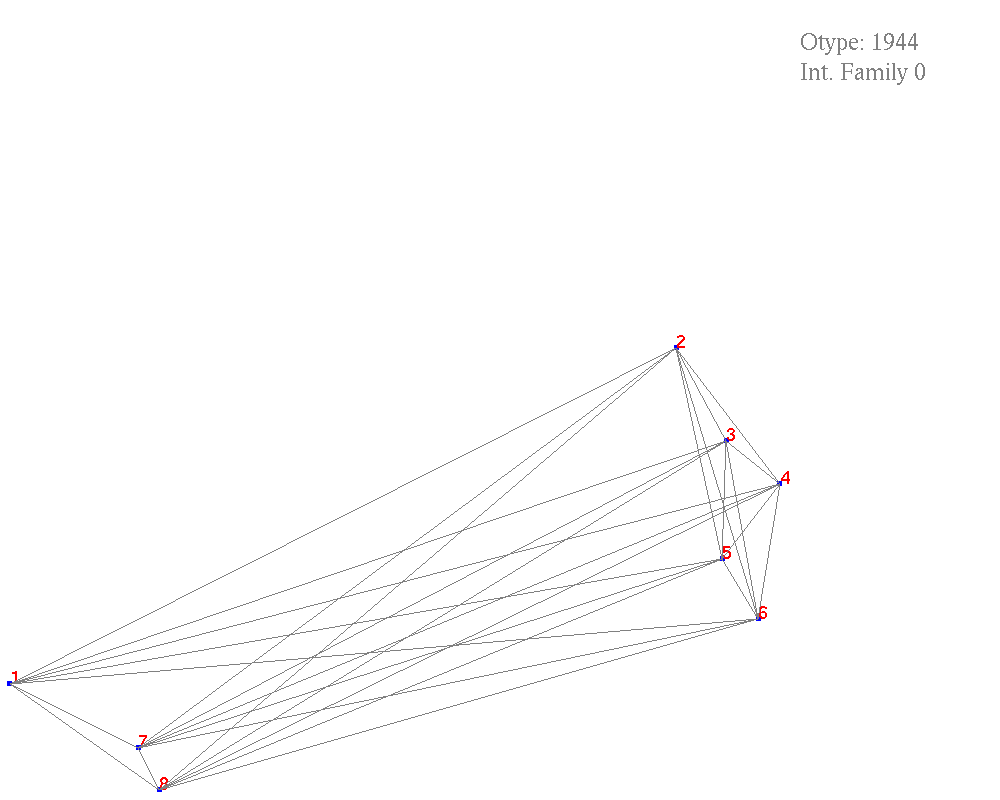
\includegraphics[scale=.4]{if_tam0_tam1/19.png}
		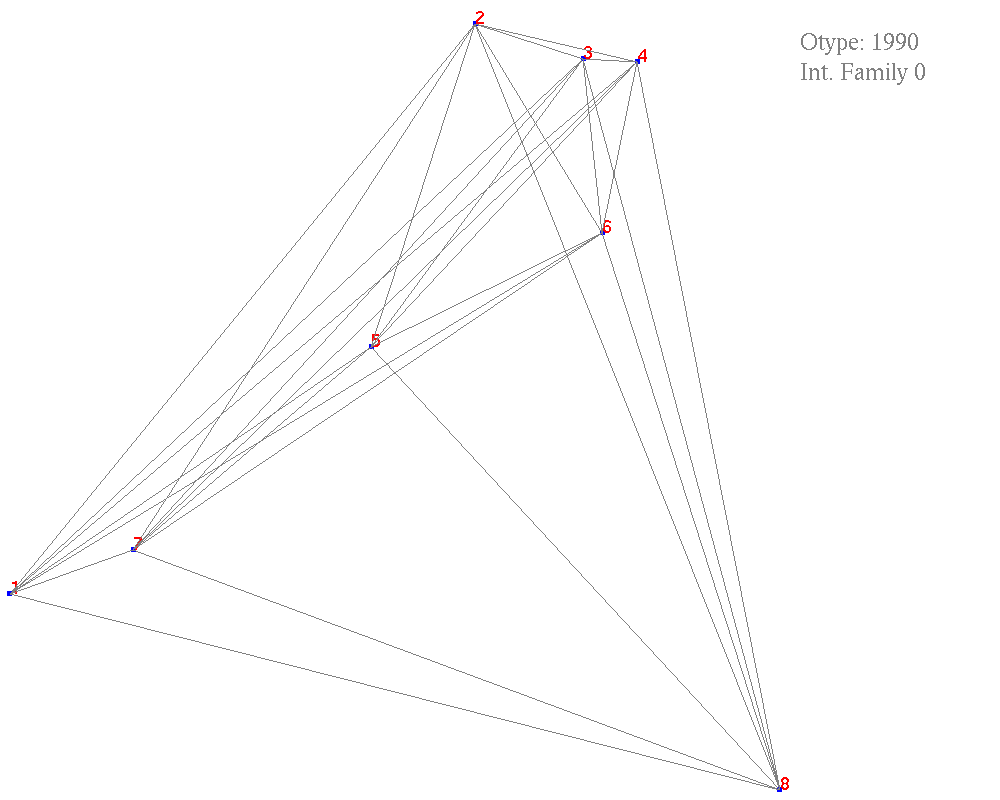
\includegraphics[scale=.4]{if_tam0_tam1/20.png}
	\end{figure}
	
	\begin{figure}
		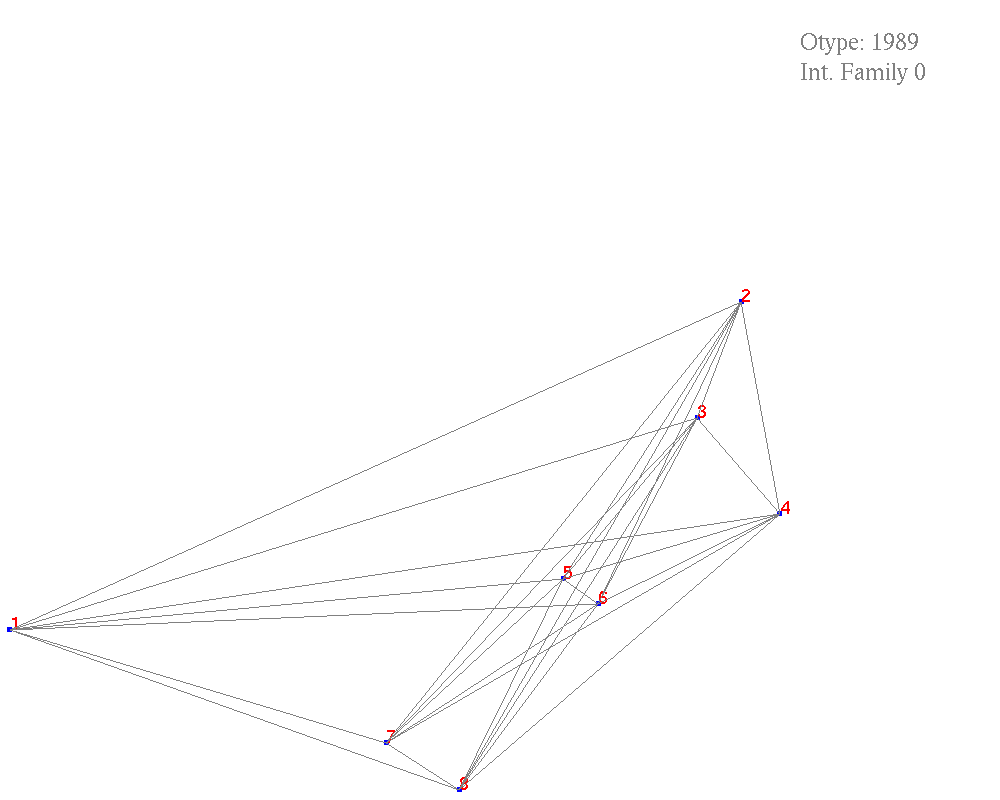
\includegraphics[scale=.4]{if_tam0_tam1/21.png}
		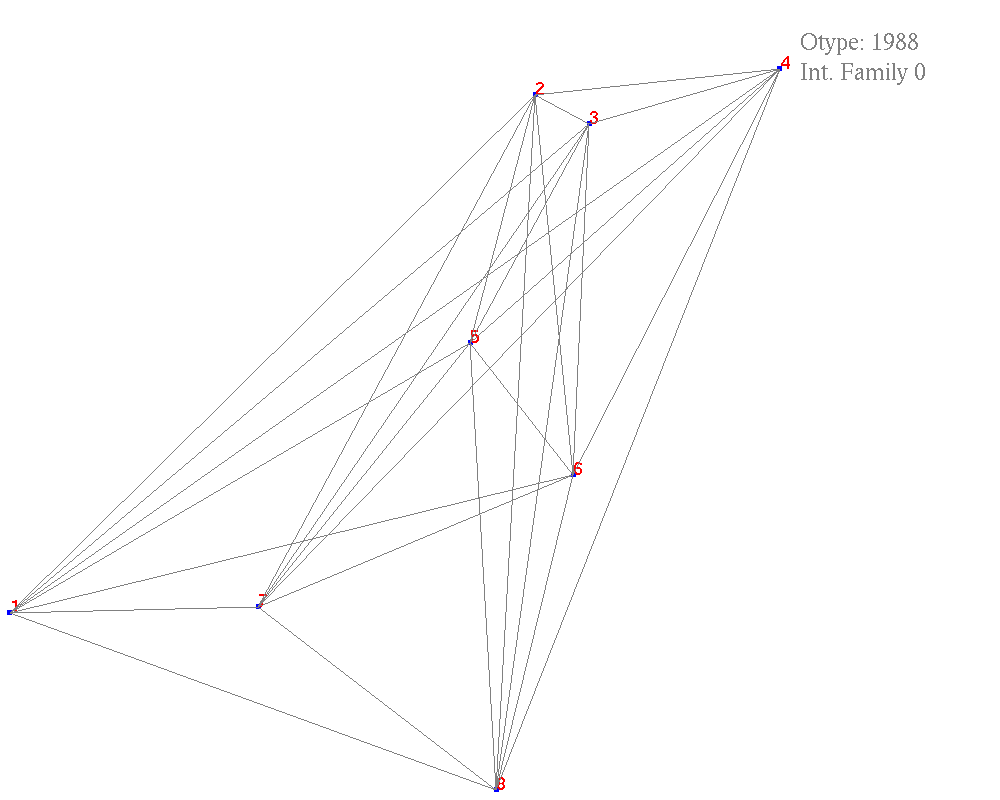
\includegraphics[scale=.4]{if_tam0_tam1/22.png}
	\end{figure}
	
	\begin{figure}
		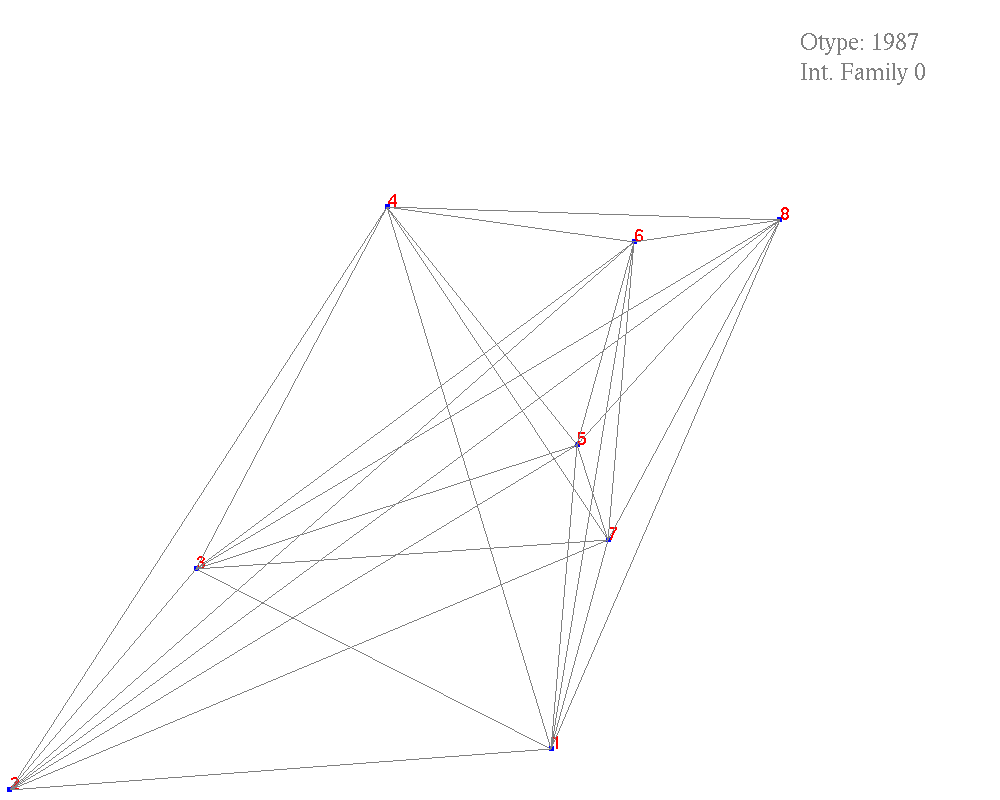
\includegraphics[scale=.4]{if_tam0_tam1/23.png}
		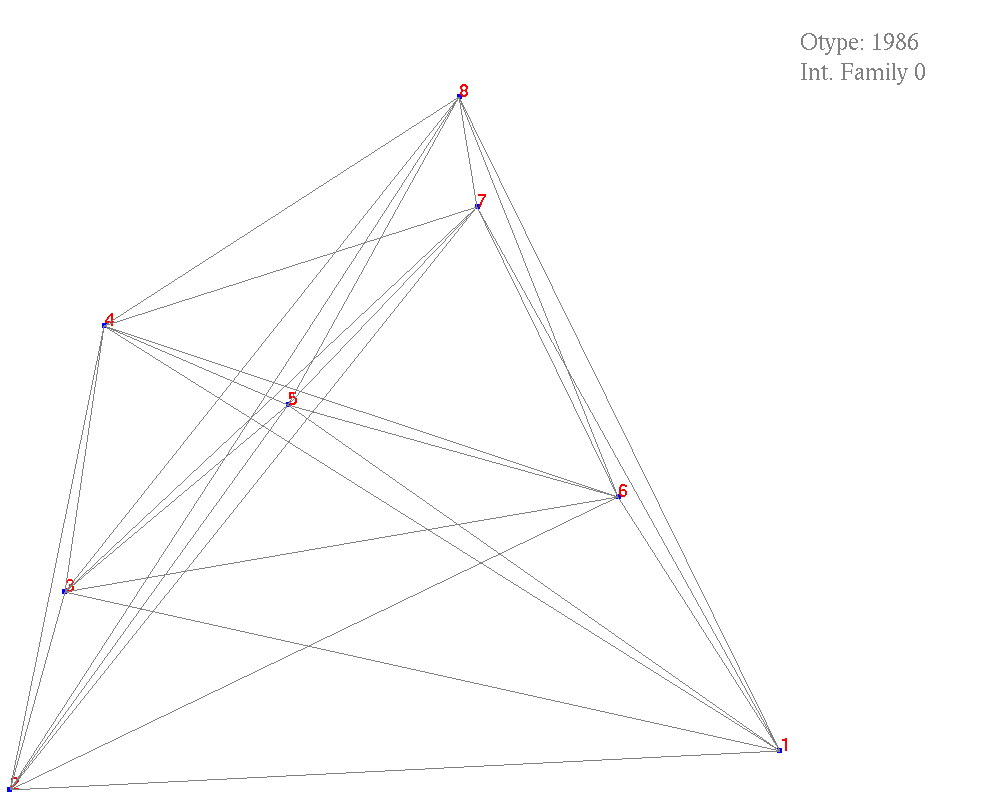
\includegraphics[scale=.4]{if_tam0_tam1/24.png}
	\end{figure}
	
	\begin{figure}
		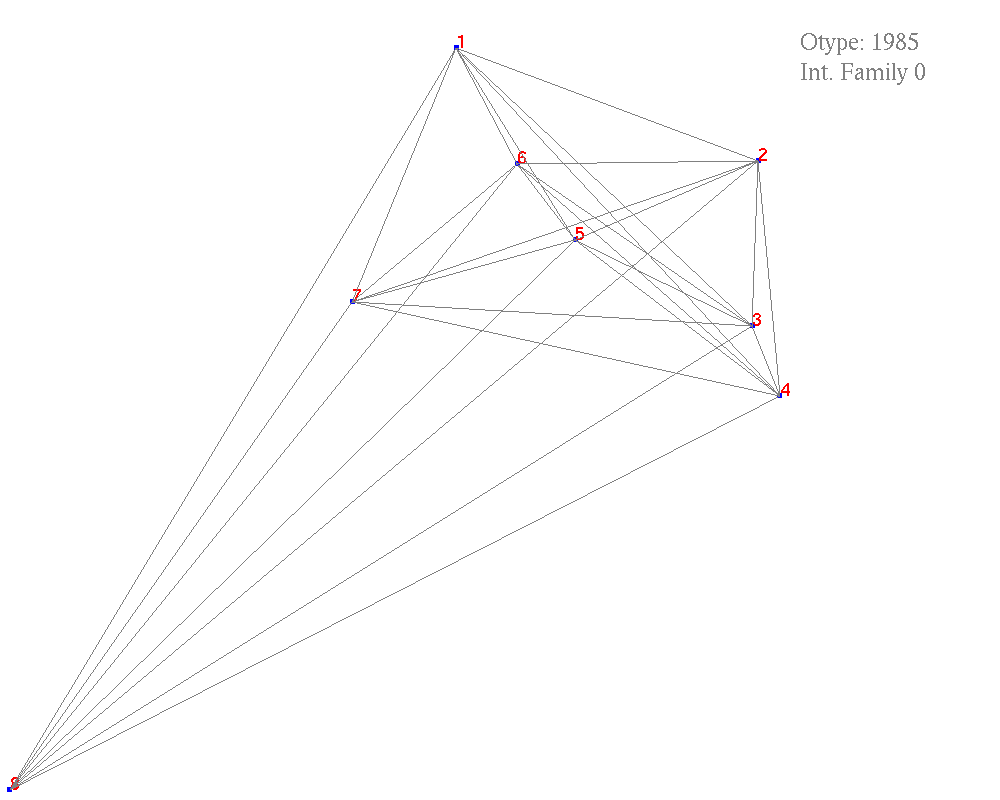
\includegraphics[scale=.4]{if_tam0_tam1/25.png}
		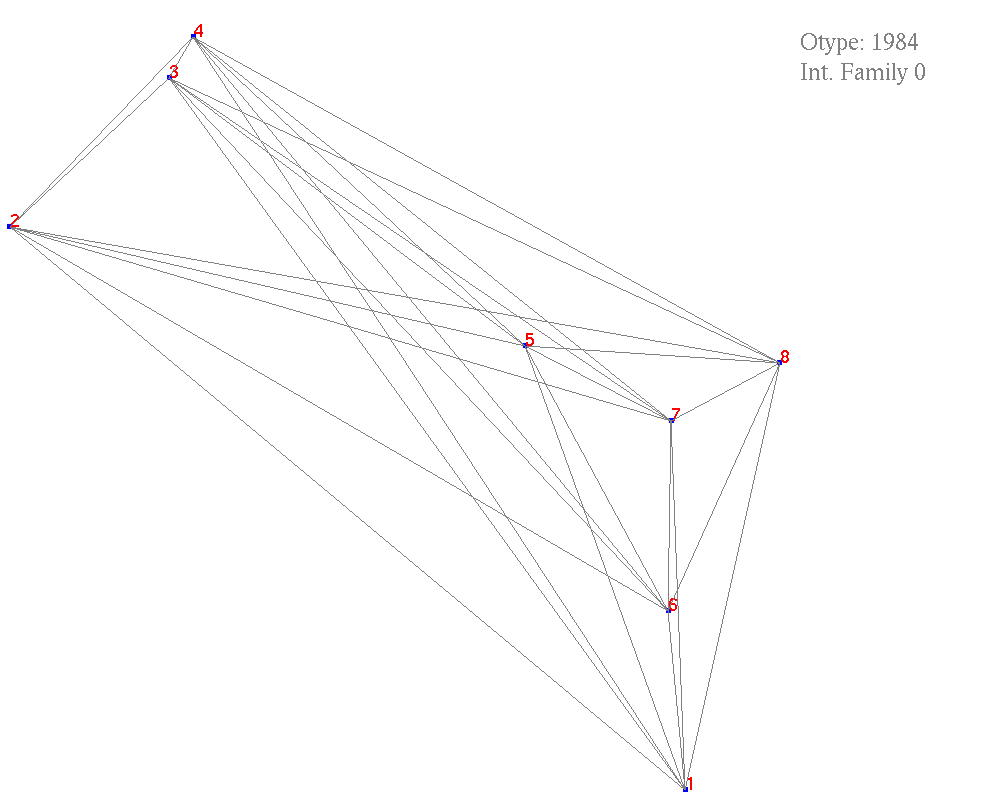
\includegraphics[scale=.4]{if_tam0_tam1/26.png}
	\end{figure}
	
	\begin{figure}
		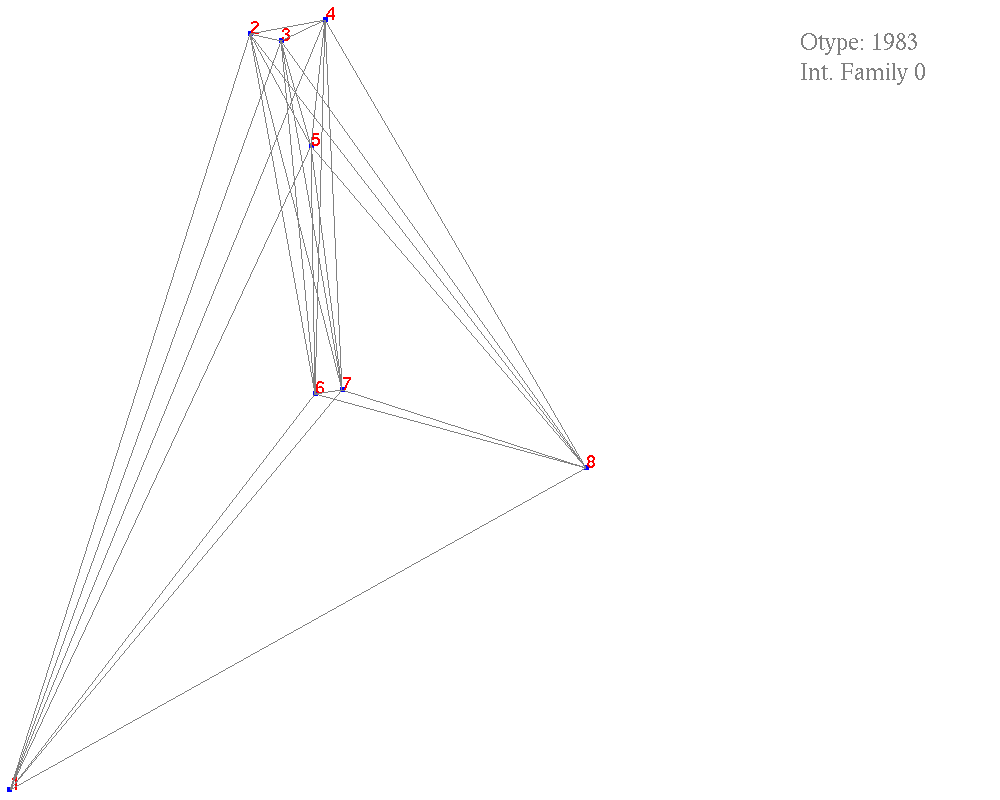
\includegraphics[scale=.4]{if_tam0_tam1/27.png}
		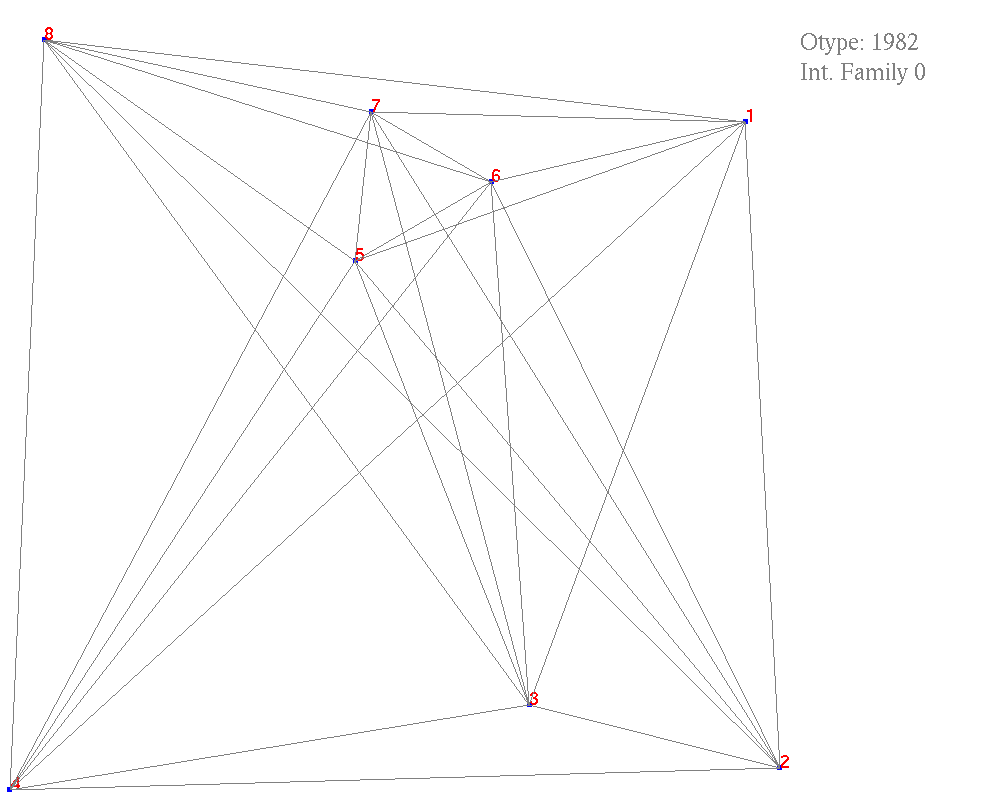
\includegraphics[scale=.4]{if_tam0_tam1/28.png}
	\end{figure}
	
	\begin{figure}
		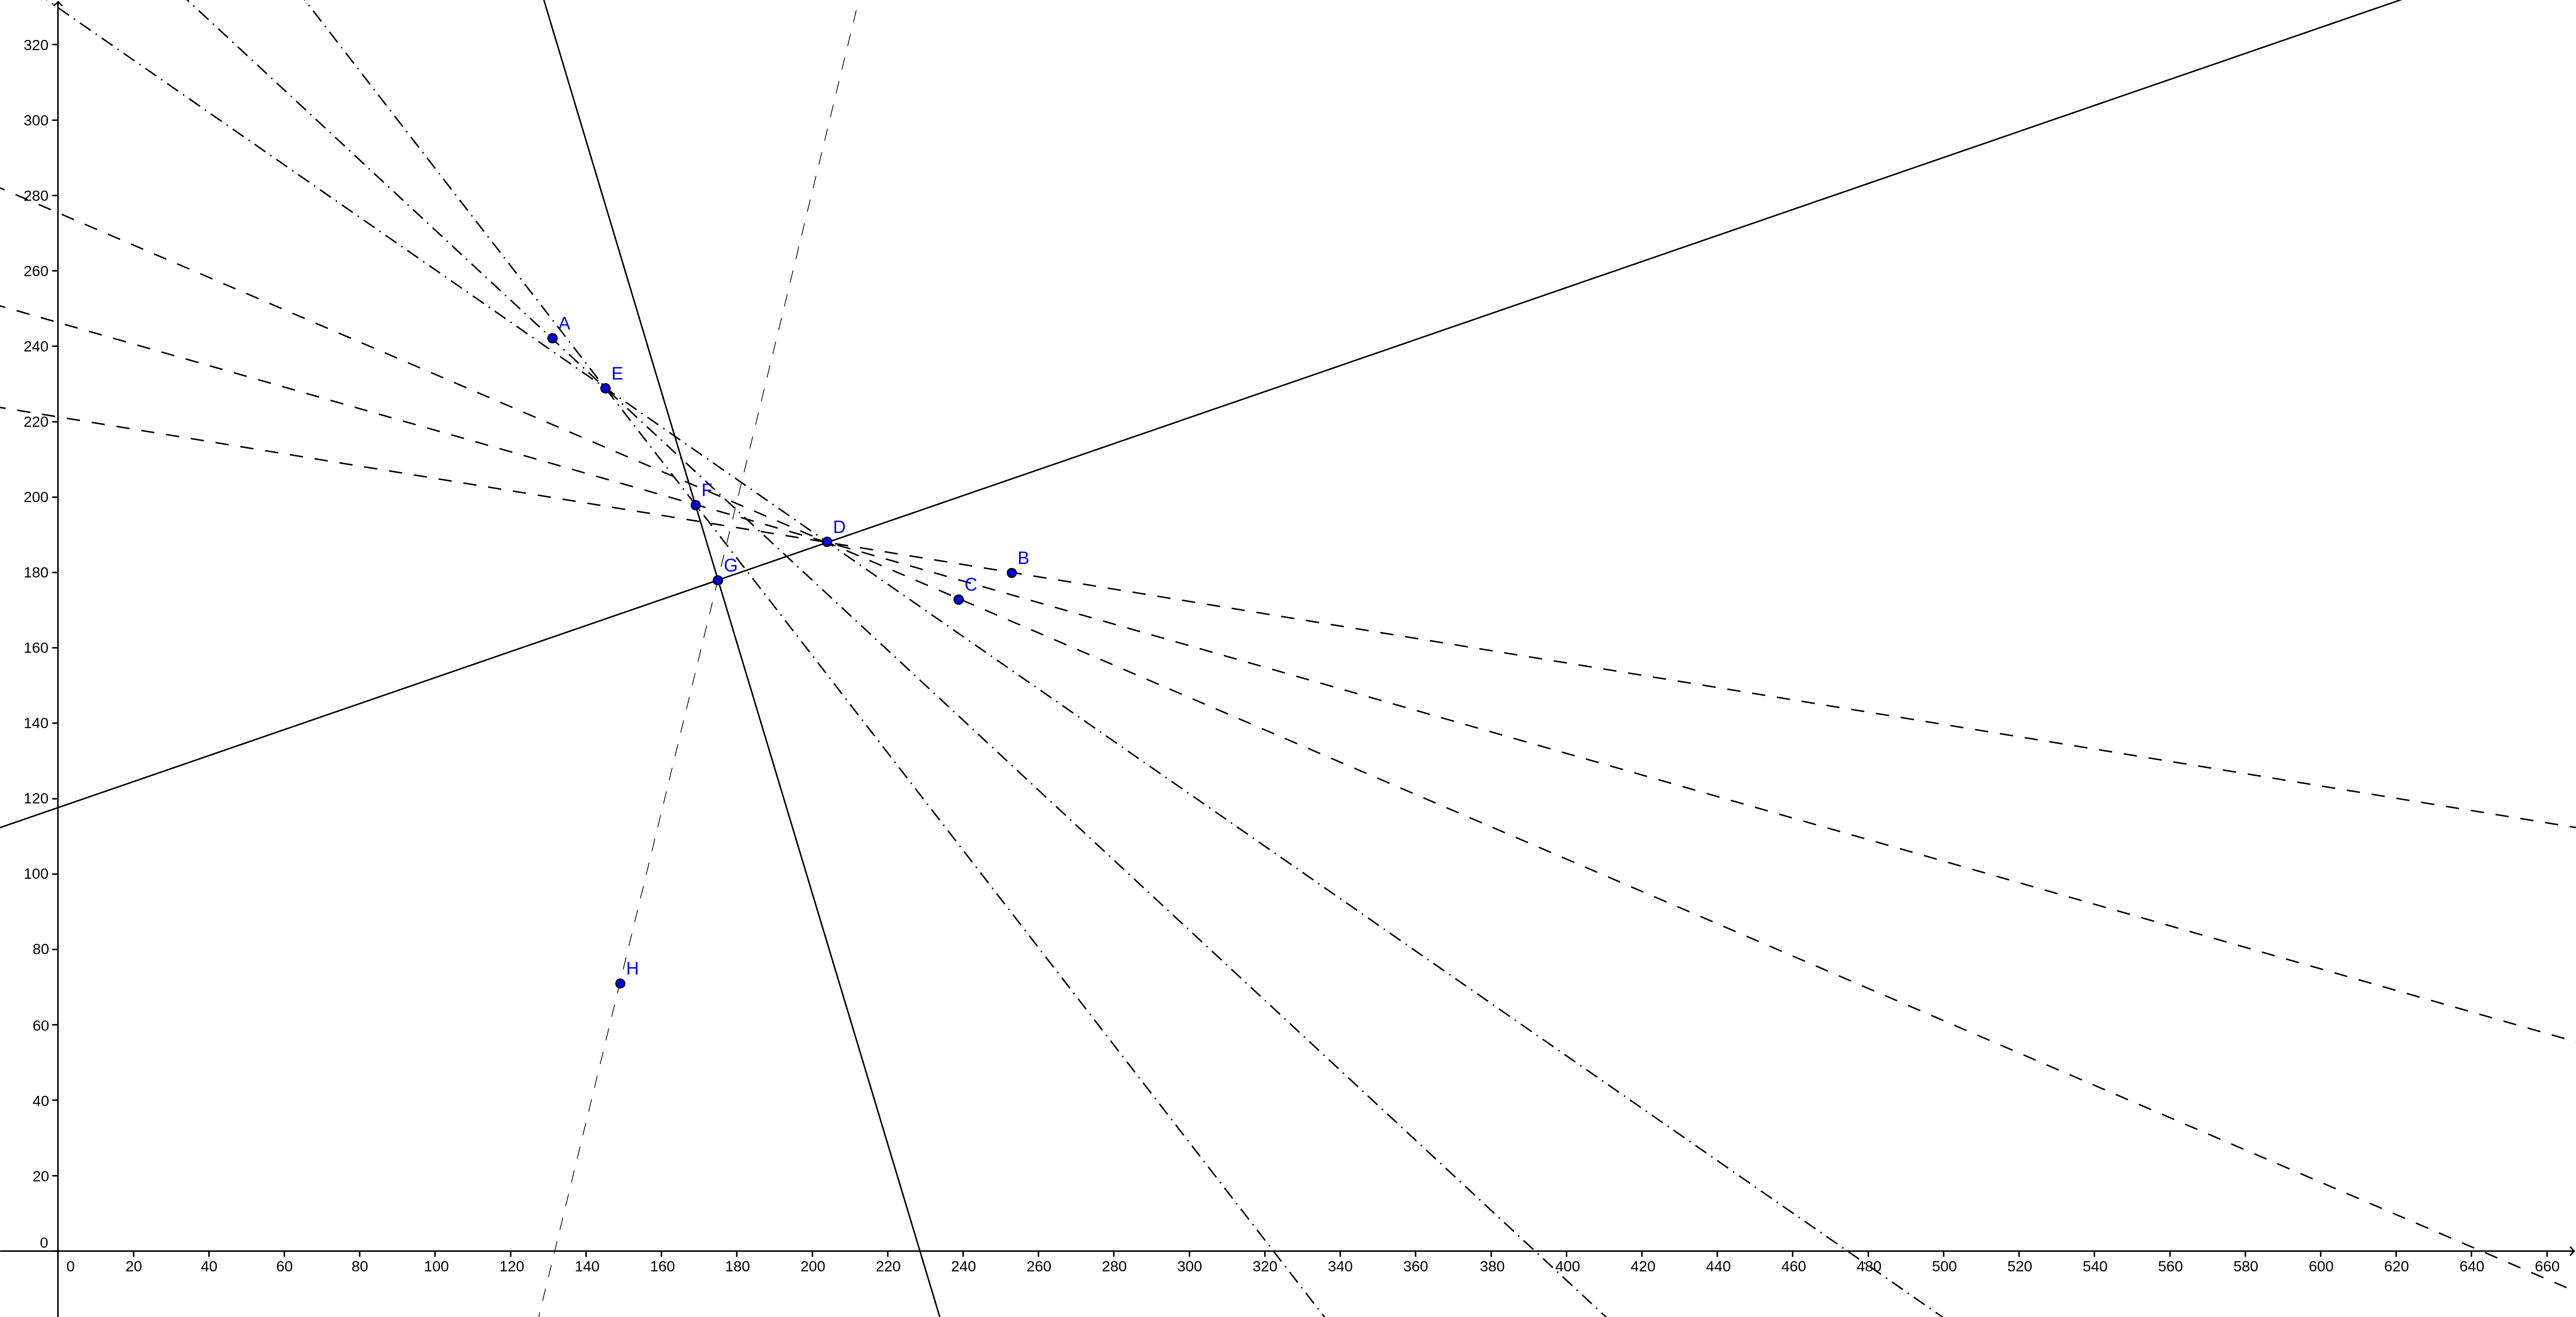
\includegraphics[scale=.35]{maxhalving_lines.png}
	\end{figure}
	
\end{document}